\documentclass[letterpaper]{article}
\usepackage{aaai}
\usepackage{times}
\usepackage{helvet}
\usepackage{courier}
\usepackage{graphicx}
% Yes, this will work with pdflatex, and not with normal latex
 \pdfinfo{
 /Title (Engineered Robustness by Controlled Hallucination)
 /Subject (AAAI Fall Symposium on Naturally Inspired AI)
 /Author (Beal, Jacob; Sussman, Gerald Jay)}

\title{Engineered Robustness by Controlled Hallucination}
\author{Jacob Beal \and Gerald Jay Sussman\\
        Massachusetts Institute of Technology}
% GJS should have first author because he's doing most of the writing?
% But Jake should be first author because he is a young man looking
% for a job -- GJS.

\begin{document}
\nocopyright
\maketitle

\begin{abstract}
  Most computer programs are brittle.  They may have acceptable
  behavior for the range of applications that they are specified to
  work for, but they fail miserably for applications even slightly
  outside of that range.  For example, a program may work well when
  its inputs are complete, but be unable to produce any sensible
  result if any of its inputs are missing or noisy.

  We propose a strategy for alleviating this kind of brittleness:
  because many programs are used repeatedly on a very sparse but
  highly structured subset of the possible inputs that might be
  provided, we can build wrappers that fill in missing or noisy data
  by inducing the missing information from the other inputs.

  We illustrate this strategy with a wrapper that acquires constraints
  on the graphical presentation of characters.  When exposed to the
  first 317 words of "Pride and Prejudice," the constraints it
  acquires capture information that can be used to fill in missing or
  clarify noisy data in similarly presented text.  This strategy of
  generalization wrappers can be applied recursively, to every
  subsystem of a large system, substantially improving the robustness
  of the system.
\end{abstract}

\section{Overview}

Hallucination is usually thought of as a perceptual failure, but it
can also be seen as a means of enhancing the robustness of a
perceptual mechanism.  Input data is invariably noisy and
incomplete, and it is usually unfamiliar.  However, there are
mechanisms that heuristically complete incomplete data, clean noise
from data, and generally make sense of unfamiliar situations by
coercing them to be more like familiar situations.  Such mechanisms
are cheaters: they construct lies.  The construction of convincing
lies appears to be a powerful mechanism of robust perception.

Inspired by this insight into the psychology of perception, we
consider the application of this idea to the enhancement of robustness
in engineered systems.  Here we develop a crude abstract model of such
a mechanism.  We have begun to test the idea in simple contexts.

\section{Communities of Specialized Parts}
% want to talk about engineered systems as well as the mind:
% dual motivation of both software & understanding cognition
% Yes, will do. -- GJS

It now seems clear that no single technique, ``general method,'' or
``unified theory'' will ever be powerful enough to account for general
intelligence, and we think it is no accident that each human brain
uses many different mechanisms, each specialized for a particular
competence.~\cite{kanwisher98,chomsky05} Minsky's
theory~\cite{societyofmind,emotionmachine} is built on exactly this
idea: that the mind is made up of agents, each implementing some
specific capability, bound together in layers.  Some of the agents are
``critics'' that modulate the behavior of other agents.  These
higher-level ``critical'' processes know or can learn multiple ways to
deal with different kinds of problems, situations, and obstacles.

% As engineers we build mechanisms, each of which is competent to solve
% some class of problems.  For example, we have mechanisms that are
% excellent at evolving the state of a system that is described by
% differential equations; so given a description of the present state we
% can predict the future of a world modeled by those equations.

In a big system there are many parts, each designed to provide some
particular feature or to deal with some particular kind of problem.
But our mechanisms are often too tightly specified: they are useful
only when the input data is complete and accurate.  This is a severe
constraint: systems built out of tightly-specified subsystems are
brittle---they fail catastrophically if the situations they are
presented with are not exactly within their specified competences.

We need new ways to integrate many different strategies into a
coherent system.  But in our present-day hardware and software
designs, if the specifications for the parts are tight enough to fully
constrain them, then those specifications will be too inflexible to
adapt to new requirements.  Traditional ``monotheistic'' theories of
software organization have proven inadequate for prescribing how to
integrate diverse subsystems into a coherent whole.  Small variations
in the problem should not entail large changes in the system.  This
kind of brittle design is all too apparent in computer systems, and in
traditional attempts to construct systems with common sense.


\section{Robustness by Hallucination}

We need to make systems that are robust in that they are useful in
circumstances not completely anticipated by their designers.  One
approach is to make each subsystem much more general than it needs to
be, so that larger than anticipated variations in the inputs to the
subsystem can be tolerated and can be expected to produce reasonable
results.  A system built out of such over-generalized subsystems can be
effective even if there is significant variation in the requirements,
because there is flexibility built in at every interface.

Although a subsystem may be sharply specified to provide a particular
competence it can often be generalized by adding a wrapper that
coerces inputs from other subsystems into a form appropriate to this
subsystem, whenever possible.  For example, suppose we have a
subsystem that performs adequately if its input data is perfect, but
there is a problem: some of its input is noisy and has occasionally
missing components.  We can attack this problem in several ways.  If
we view missing or noisy data as uncertainty we are led to
probabilistic methods.  Alternatively, we can build mechanisms that
try to complete the missing or noisy data.  Although some of these
completions will be inappropriate, the cost of being occasionally
misled may be greatly outweighed by the cost of working with
inconsistent data.

Illusions provide some insight into these mechanisms.  Humans
regularly ``see'' lines that are not actually present in a visual
scene.  Kanizsa's triangle
illusion~\cite{kanizsa79,gregory77,nieder02} is a spectacular
demonstration of this phenomenon.  Apparently there are mechanisms
that ``hallucinate'' the missing features for the mechanisms that we
have for parsing scenes.

We propose a general strategy, based on controlled hallucination,%
\footnote{This idea has numerous antecedents.  

  ``Creative repetition is of course one of the central principles of
  all criticism, which has held for many centuries that poetry
  presents a kind of controlled hallucination: something in the past,
  normally accessible only to the memory, is brought into the present
  by the imagination.''~\cite{frye}

  Jan~Koenderink and Andrea~van~Doorn~\cite{Koenderink08} have
  explored a rather formal analysis of the constraints of geometrical
  structure on the structure of visual spaces.  They think of the
  guesses that a visual system must make to extract depth information
  from monocular depth cues as controlled hallucination, analogous
  to analysis by synthesis in computer vision.~\cite{ullman}}
for self-configuring wrappers that extend the range of applicability
of subsystems to cases that they were not designed or specified to
work in, at the cost of producing some incorrect results in
unspecified situations.  However such systems can often produce
reasonable behavior in situations that would otherwise lead to a
catastrophic failure.

\section{The Idea in a Nutshell}

Suppose that we want to extend the range of applicability of some
specialized but competent expert subsystem.  The job of the subsystem
is to perform actions based on its stream of inputs.  The particular
action taken at each moment depends on the recent history of the
stream.  If an input is noisy or contains some missing components, the
subsystem will be unable to produce a reasonable response.

Our wrapper will observe the stream of inputs and capture common
patterns from the history.  When a bad input appears, if there is a
captured pattern that matches the good components of the input and the
relevant parts of the current history, the wrapper will produce a
patch to the input that fills in the missing or bad data with an
appropriate hallucination.

How do we make such a wrapper?  How does it ``learn'' the appropriate
patterns?  What does it need to work usefully?  This idea will make
sense only when the possible set of input data streams is vastly
larger than the set of input streams that can actually appear, because
of unmodeled constraints in the source of the data.  These constraints
will show up as clustering of the sparse data.  The power of our idea
is to experimentally extract some of these unmodeled constraints and
exploit the redundancy and sparseness so discovered as
error-correcting codes.


\subsection{A first approximation}

Assume for the moment that the inputs are tuples of symbols chosen
from finite sets.  Assume also, for the moment, that some of the
tuples from the product set will produce a reasonable output from the
subsystem and others will not.  For example, some argument symbols can
represent missing or noisy data.

We build a wrapper that intercepts the input tuples before presenting
them to the subsystem.  It also observes whether the subsystem is
happy with those inputs.  The wrapper deterministically generalizes on
the tuples that produced acceptable or unacceptable outputs, by a
mechanism that we will explain.  When the wrapper receives a tuple
that it thinks will be unacceptable, it perturbs that tuple to be one
that is acceptable, perhaps by filling in missing data in a way that
is consistent with its previous experience, and passes the perturbed
tuple to the expert subsystem.

The idea, as described above, can only fill in missing or noisy data
based on the current input tuple.  But this scheme can be expanded to
deal with time series.  For example, if our wrapper buffers input
tuples with a shift register~\cite{DBLP:conf/aaai/YipS97}
then patterns of past behavior can be used to fill in missing data in
the present.  But more: information from the present can be used to
fill in missing data in the past, and if the shift register also
contains some slots for the future, predictions can be made that may
be useful when that future comes to pass.  Indeed, past, present, and
future data all can be simultaneously refined.

Unfortunately, the shift register idea depends on a uniform scale of
time.  We cannot make correlations over very long periods if we also
want to make detailed short-term correlations.  However, if we use
more scale-invariant representations, such as Allen's
relations~\cite{allen83}, and if we concentrate on
changes~\cite{borchardt}, we get powerful abstractions of the history
that can work on multiple time scales.

% illustration of a shift register

\subsection{An example mechanism}

Let's start with a shift-register example.  Each data tuple element
(a ``feature'') is allocated one row of the register.  The columns of
the register correspond to moments.  So each entry in the register
holds the value of a feature at a recent moment.

Data tuples from the inputs are entered into the ``current moment''
column of the shift register.  There are columns after the current
moment (the ``past'' and before the current moment (the ``future'').  The
future moments are initialized to a value that may be overridden with
real data.  We will see how those are used later.

Entries from the shift register are observed by subsystems that need
its data.  If a subsystem cares about only data at a particular moment
it looks at features in exactly one column of the register.  If it is
interested in the evolution of some features it may sample features
from several columns.  We assume that past columns extend beyond the
point where any subsystems are observing.

Now, here's the trick.  Let many subsets of the entries from the shift
register, from some rows and some columns, be selected (perhaps
randomly?).  For each such subset a data structure is allocated (a
{\em correlator} memory) to hold the identities of the entries and the
values currently in those entries.  For each subsequent moment, for
each of these correlators, its remembered values are compared with the
current values in its entries.  If almost all of the values match, the
correlator forces the value in the discrepant entries in the shift
register to have the values previously remembered.  The correlator
also signs those values it changes with its identity.  If a subsystem
using this shift register finds its inputs unacceptable, and if any of
the unacceptable values is traceable to a particular correlator, that
correlator is ``killed.''  It is cleared and deallocated and a new subset
is chosen and a new correlator is allocated.

Some correlator subsets may include entries in the shift register that
are in the future---before the current moment column.  These special
entries are initialized in a correlator that references them to values
that appear in the current column, delayed by the number of shifts
that the entry is in the future.  Thus, a correlator may make a
prediction about the future.  Indeed, if such a prediction is
contradicted by the evidence coming in from the inputs a correlator
that makes the erroneous prediction is killed.

Of course, this is an idealized description; the reality is more
complex.  How big is the shift register?  How big are the subsets?
How many are they?  What does ``almost all'' mean?  There are a few
parameters that determine the performance of such a system.


\section{An Experiment}

To investigate this idea we have built a computational apparatus for
experimenting with streams of characters, rendered as pixels.  This is
a nice medium for experiments because it is clear what a character
should look like, and it is easy to introduce noise, missing data, and
distortions into the stream.  

However, there are some complications.  We don't want to deal with the
pixels as the primary features of the rendered characters, because
they are not shift invariant, with respect to vertical position, and
they are not scale invariant.  We also want to limit the size of the
feature set so that our experiments could be performed without massive
computational resources.

%      P  r     e     j
% ..................._....
% ..................._....
% ..........._________S...
% ........____________....
% ....________________L...
% ...._________RFF____-...
% ____________H___MS_H_...
% _________R_M_HHH_____...
% _____H______FFFHH____...
% ______M_L____________...
% RSL_LH_______________...
% _____________________...
% ................_____...

%  j  u    d   i   c
% ____________________....
% ____________________....
% _S__________________....
% _________RSL_S______....
% _L_L__L_M_______RS__....
% _________FS__L_M____....
% H___FR__________FS_M....
% ____________________-...
% ____________________....
% ____________________....
% ..............______....
% ..............______....
% .................___....

\begin{figure}
\centering
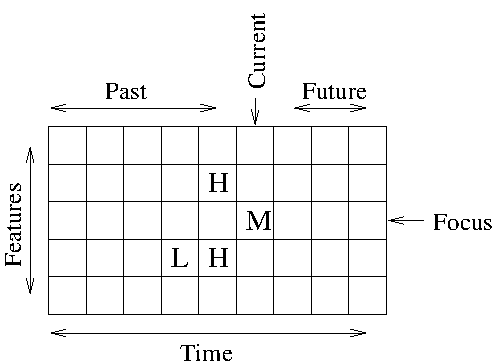
\includegraphics[width=3in]{shift.pdf}
\caption{The register shifts from right to left.  Current information
  is entered at the column marked {\tt current}, overwriting any
  predictions entered in the future columns by correlators with
  fingers in the future.  The features representing the letter ``P''
  have just been entered into the shift register.  The last feature
  entered is {\tt M} (for the {\tt Medium} vertical line on the right side of
  the ``P'').  It is in the focus slot of the current column.}
\label{fig:shift}
\end{figure}

The representation we chose is based on a window that moves across the
characters in the stream from left to right.  As the window slides
along, vertical slices of pixels are progressively assembled together
to form lines that interpreted as approximately horizontal, rising,
falling, or one of three vertical sizes.  For example, consider the
letter ``P.''  First a {\tt Large} vertical line appears.  Two
approximately {\tt Horizontal} lines come out of it, at the top and
middle.  Before these lines have curved enough to seriously depart
from the horizontal, they terminate going into the top and bottom of a
{\tt Medium} approximately vertical line.  These features and a few
others are the analog of the ``distinctive features'' that are found
in the study of phonology.

These features are shifted into our shift register. (See
figure~\ref{fig:shift}.)  A new shift occurs {\em only} when a change
occurs in the sort of lines appearing in our window.  This provides a
kind of invariance with respect to the actual width of the characters
in the pixel raster.  Also, a changed feature becomes a focus of
attention.  If more than one changes, the bottom change becomes the
principal focus.  The features are shifted vertically before being
shifted into the register so that the principal focus is always in a
fixed position of the register.  This provides a kind of invariance
with respect to vertical position of the characters on the pixel
raster.  Finally, each new feature is placed in a fixed position with
respect to the lines already being tracked, thus making the
representation invariant with respect to vertical scale on the pixel
raster, so long as an approximate scale is specified to allow the type
of vertical line to be determined and to distinguish small verticals
from short horizontals.

Our mechanism entails an interesting complication.  Because the focus
of attention is always at a particular feature position in the shift
register, the determination of which future feature corresponds to a
current feature (for prediction) depends on keeping track of the
number of vertical (feature) shifts occur in the horizontal (time)
shifts that bring the to-be-predicted future to the present.

\begin{figure}
\centering
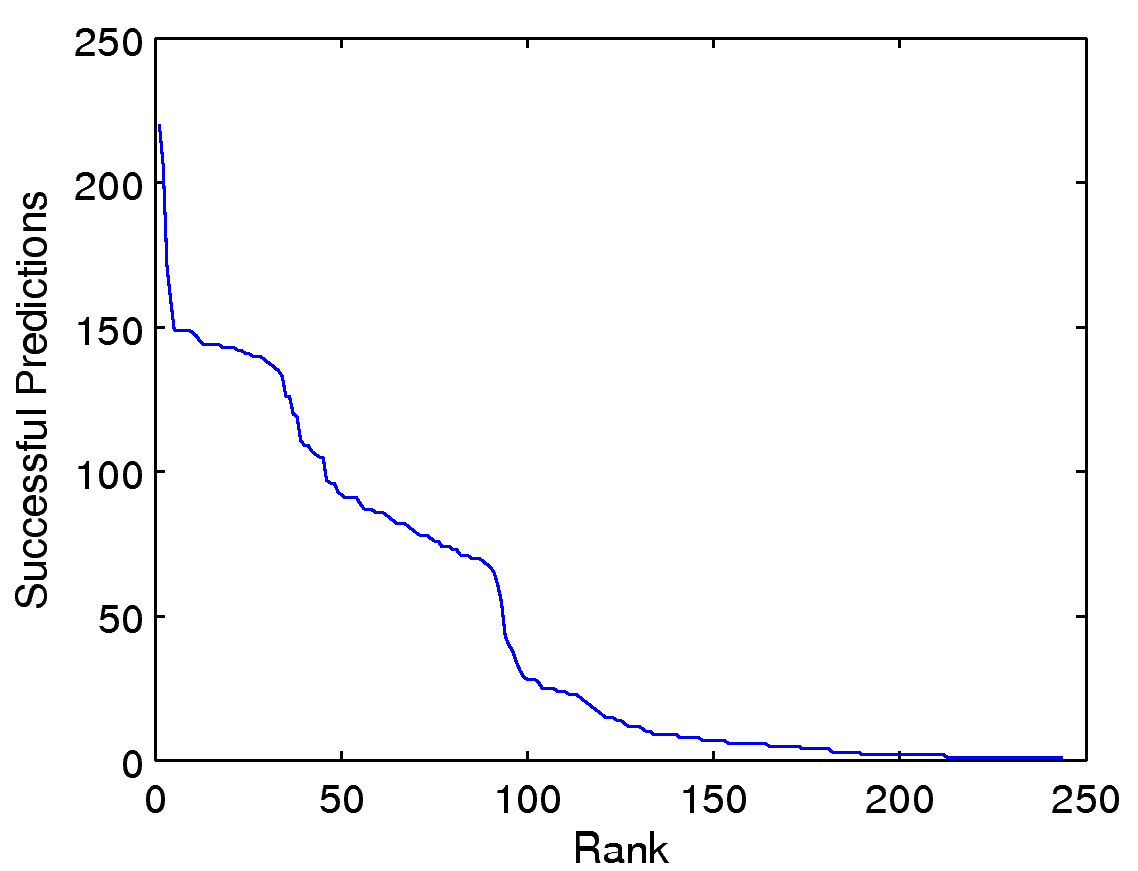
\includegraphics[width=3in]{austen.png}
\caption{After a population of 1000 correlators is exposed to the
  first 317 words of ``Pride and Prejudice,'' 244 of the survivors
  have made at least 1 correct prediction without any failures, 133
  have made at least 10, and 45 have made at least 100.}
\label{f:results}
\end{figure}

% continue revising here
We have built this mechanism, and our first test of its efficacy was
to expose a population of 1000 correlators to the first 317 words of
Jane Austen's ``Pride and Prejudice.''  As anticipated, we find that
the population of correlators has acquired patterns that capture
interesting structure in English text.  Figure~\ref{f:results} shows
the distribution of number of correct predictions in the subpopulation
of 244 correlators that have at least one correct prediction at the
end of the exposure.  Nearly 5\% of the correlators have predicted
their current pattern 100 times without failure.  These extremely
strong patterns generally relate to 'e', 'a', or 's'---letters that
are both complicated and common, making them easy targets for
learning.  Other letters are represented as well, with lower numbers
of successful predictions, such as 'g', 'i', 'f', 'y.'  There are even
multi-letter patterns, such as one that matches 'as' and another that
matches an 'i' following a downward arc, such as 'hi', 'ni', 'gi' and
'mi.'

These results indicate that we the mechanism is working as predicted
and should be able to be used to repair missing or incorrect
information.  More work is necessary to answer questions about the
mechanism, such as: How many correlators will be needed?  How many
features should they look at?  The next obvious test is to add noise
to the data and see how well our mechanism can repair the damage.
Finally, one could render our corpus in a different font and see how
many of the correlators that provided useful work with the first font
can survive the transformation.

% First N 10+ predictors:
%  0 = e,  2 = e,  3 = e,  4 = e,  7 = e
%  9 = s, 11 = e, 12 = e, 16 = e, 17 = e
% 20 = a, 23 = a, 26 = s, 27 = e, 31 = e
% 33 = a, 35 = e, 36 = s, 43 = s, 45 = s

% 217 = hi/ni/gi/mi
% 302 = f
% 565 = i
% 656 = g
% 685 = g
% 688 = y
% 694 = as
% [actually, lots of g]


\section{Conclusion}

In this position paper we propose a rather simple but dirty way of
extending the range of applicability of a subsystem so that it can
usefully accept noisy or incomplete data.  Of course there are other,
more principled, ways of dealing with uncertainty.  For example, one
can try to explicitly represent the uncertainty and use probabilistic
methods to obtain best estimates of the values of missing parameters
in the face of uncertain information.  Even more conservative
mechanisms may keep all possible alternatives in hand and discard an
alternative only after it is contradicted by reliable
information~\cite{waltz}. However, quick-and-dirty mechanisms that
wish away uncertainty by manufacturing possible completions may be
quite effective in some contexts.

This is only one of many ideas that were originally inspired by
observation of natural intelligence and developed into software
techniques for experiments in artificial intelligence that may have
wider applicability in engineering design.

\bibliography{main}
\bibliographystyle{aaai}

\end{document}
